\subsubsection{Lan truyền tiến}
Về cơ bản quy trình huấn luyện mạng nơ-ron truyền thẳng gồm hai pha tuần tự: 
\begin{enumerate}
    \item \textit{Lan truyền tiến:} Dữ liệu đầu vào được truyền một chiều qua các lớp ẩn đến lớp đầu ra để tạo giá trị dự đoán.
    
    \item \textit{Lan truyền ngược:} Đánh giá mức độ sai lệch giữa giá trị dự đoán và giá trị thực tế thông qua hàm mất mát, từ đó áp dụng quy tắc chuỗi để tính các gradient của hàm mất mát theo từng tham số ngược từ lớp đầu ra về lớp đầu vào.
\end{enumerate}

Nhằm đảm bảo tính nhất quán trong ký hiệu toán học xuyên suốt mạng nơ-ron, véc-tơ đặc trưng đầu vào được quy ước là véc-tơ kích hoạt của lớp $0$, ký hiệu là $\mathbf{a}^{[0]} \in \mathbb{R}^{n_0}$:
\begin{equation}
    \mathbf{a}^{[0]} = \begin{bmatrix} a_1^{[0]} & a_2^{[0]} & \dots & a_{n_0}^{[0]} \end{bmatrix}^\top,
\end{equation}
trong đó $n_0$ là số lượng chiều (đặc trưng) của dữ liệu đầu vào.

Giả sử mạng nơ-ron truyền thẳng bao gồm $L$ lớp (không tính lớp đầu vào $l=0$), trong đó mỗi lớp thứ $l$ (với $1 \le l \le L$) chứa $n_l$ nơ-ron. Lớp cuối cùng $L$ được gọi là lớp đầu ra. Tại một lớp $l$ bất kỳ, ta định nghĩa các đại lượng không gian tham số như sau:
\begin{equation}
\begin{aligned}
    \mathbf{W}^{[l]} &= \begin{bmatrix}
        w_{11}^{[l]} & w_{12}^{[l]} & \dots & w_{1, n_{l-1}}^{[l]} \\
        w_{21}^{[l]} & w_{22}^{[l]} & \dots & w_{2, n_{l-1}}^{[l]} \\
        \vdots & \vdots & \ddots & \vdots \\
        w_{n_l 1}^{[l]} & w_{n_l 2}^{[l]} & \dots & w_{n_l, n_{l-1}}^{[l]}
    \end{bmatrix} \in \mathbb{R}^{n_l \times n_{l-1}}, \\
    \mathbf{a}^{[l]} &= \begin{bmatrix} a_1^{[l]} \\ a_2^{[l]} \\ \vdots \\ a_{n_l}^{[l]} \end{bmatrix} \in \mathbb{R}^{n_l}, \quad
    \mathbf{b}^{[l]} = \begin{bmatrix} b_1^{[l]} \\ b_2^{[l]} \\ \vdots \\ b_{n_l}^{[l]} \end{bmatrix} \in \mathbb{R}^{n_l}.
\end{aligned}
\end{equation}
Trong đó:
\begin{itemize}
    \item $l$: Biến chỉ số biểu diễn thứ tự của lớp đang xét, $l \in \{1, 2, \dots, L\}$.
    \item $n_l$: Số lượng đơn vị tính toán tại lớp thứ $l$. Tương ứng, $n_{l-1}$ là số lượng đơn vị tại lớp liền trước.
    \item Chỉ số trên ngoặc vuông $[l]$: Quy ước chỉ số thứ tự của lớp tính toán trong mạng nơ-ron. Ở đây, $[0]$ biểu thị lớp đầu vào.
    \item $\mathbf{W}^{[l]}$: Ma trận trọng số kết nối từ lớp $l-1$ sang lớp $l$.
    \item $w_{ij}^{[l]}$: Phần tử nằm trên hàng $i$, cột $j$ của ma trận $\mathbf{W}^{[l]}$. Giá trị này định lượng mức độ ảnh hưởng (trọng số liên kết) của tín hiệu từ nơ-ron thứ $j$ thuộc lớp $l-1$ truyền tới nơ-ron thứ $i$ thuộc lớp $l$.
    \item $\mathbf{a}^{[l]}$: Véc-tơ kích hoạt (đầu ra) của lớp $l$.
    \item $\mathbf{b}^{[l]}$: Véc-tơ độ chệch của lớp $l$.
    \item $b_i^{[l]}$: Hệ số độ chệch tương ứng với nơ-ron thứ $i$ tại lớp $l$.
\end{itemize}
Tại mỗi lớp $l$, quá trình lan truyền tiến được mô tả qua hai bước. Đầu tiên, véc-tơ tiền kích hoạt $\mathbf{z}^{[l]}$ được tính thông qua một phép biến đổi tuyến tính:
\begin{equation}
    \mathbf{z}^{[l]} = \mathbf{W}^{[l]} \mathbf{a}^{[l-1]} + \mathbf{b}^{[l]}
\end{equation}
Sau đó, véc-tơ kích hoạt $\mathbf{a}^{[l]}$ được tính bằng cách áp dụng một hàm kích hoạt $\sigma^{[l]}$ lên véc-tơ $\mathbf{z}^{[l]}$:
\begin{equation}
    \mathbf{a}^{[l]} = \sigma^{[l]}(\mathbf{z}^{[l]})
\end{equation}
Trong đó, $\sigma^{[l]}(\cdot)$ là hàm kích hoạt của lớp $l$, tác động độc lập theo từng phần tử lên thành phần đầu vào của nó.

Để làm rõ bản chất đại số, ta khai triển chi tiết phép tính cho véc-tơ tiền kích hoạt $\mathbf{z}^{[l]}$:
\begin{equation}
\begin{aligned}
    \mathbf{z}^{[l]} &= \mathbf{W}^{[l]} \mathbf{a}^{[l-1]} + \mathbf{b}^{[l]} \\
    &= \begin{bmatrix}
        w_{11}^{[l]} & w_{12}^{[l]} & \dots & w_{1, n_{l-1}}^{[l]} \\
        w_{21}^{[l]} & w_{22}^{[l]} & \dots & w_{2, n_{l-1}}^{[l]} \\
        \vdots & \vdots & \ddots & \vdots \\
        w_{n_l 1}^{[l]} & w_{n_l 2}^{[l]} & \dots & w_{n_l, n_{l-1}}^{[l]}
    \end{bmatrix}
    \begin{bmatrix}
        a_1^{[l-1]} \\
        a_2^{[l-1]} \\
        \vdots \\
        a_{n_{l-1}}^{[l-1]}
    \end{bmatrix}
    +
    \begin{bmatrix}
        b_1^{[l]} \\
        b_2^{[l]} \\
        \vdots \\
        b_{n_l}^{[l]}
    \end{bmatrix} \\
    &= \begin{bmatrix}
        w_{11}^{[l]} a_1^{[l-1]} + \dots + w_{1, n_{l-1}}^{[l]} a_{n_{l-1}}^{[l-1]} + b_1^{[l]} \\
        w_{21}^{[l]} a_1^{[l-1]} + \dots + w_{2, n_{l-1}}^{[l]} a_{n_{l-1}}^{[l-1]} + b_2^{[l]} \\
        \vdots \\
        w_{n_l 1}^{[l]} a_1^{[l-1]} + \dots + w_{n_l, n_{l-1}}^{[l]} a_{n_{l-1}}^{[l-1]} + b_{n_l}^{[l]}
    \end{bmatrix} \\
    &= \begin{bmatrix}
        \sum_{j=1}^{n_{l-1}} w_{1j}^{[l]} a_j^{[l-1]} + b_1^{[l]} \\
        \sum_{j=1}^{n_{l-1}} w_{2j}^{[l]} a_j^{[l-1]} + b_2^{[l]} \\
        \vdots \\
        \sum_{j=1}^{n_{l-1}} w_{n_l j}^{[l]} a_j^{[l-1]} + b_{n_l}^{[l]}
    \end{bmatrix}
    = \begin{bmatrix}
        z_1^{[l]} \\
        z_2^{[l]} \\
        \vdots \\
        z_{n_l}^{[l]}
    \end{bmatrix}
\end{aligned}
\label{f-z}
\end{equation}
Véc-tơ kích hoạt tương ứng được tính bằng cách áp dụng hàm kích hoạt lên từng phần tử của véc-tơ tiền kích hoạt:
\begin{equation}
\begin{aligned}
    \mathbf{a}^{[l]} &= \sigma^{[l]}(\mathbf{z}^{[l]}) \\
    &= \begin{bmatrix}
        \sigma^{[l]}\left(z_1^{[l]}\right) \\
        \sigma^{[l]}\left(z_2^{[l]}\right) \\
        \vdots \\
        \sigma^{[l]}\left(z_{n_l}^{[l]}\right)
    \end{bmatrix}
    = \begin{bmatrix}
        a_1^{[l]} \\
        a_2^{[l]} \\
        \vdots \\
        a_{n_l}^{[l]}
    \end{bmatrix}.
\end{aligned}
\end{equation}
Nhằm tinh gọn việc biểu diễn không gian tham số, mỗi hệ số độ chệch $b_i^{[l]}$ ở lớp $l$ được quy ước đóng vai trò như một trọng số liên kết ứng với đơn vị đầu vào thứ $0$ của ma trận trọng số tại lớp $l$, ký hiệu là $w_{i0}^{[l]}$. Dưới góc độ này, véc-tơ độ chệch $\mathbf{b}^{[l]}$ tại lớp $l$ được đồng nhất hoàn toàn với véc-tơ trọng số $\mathbf{w}_0^{[l]}$:
\begin{equation}
    \mathbf{b}^{[l]} = \mathbf{w}_0^{[l]} = \begin{bmatrix} 
        w_{10}^{[l]} \\ 
        w_{20}^{[l]} \\ 
        \vdots \\ 
        w_{n_l 0}^{[l]} 
    \end{bmatrix} \in \mathbb{R}^{n_l}.
\end{equation}
\begin{figure}[H]
    \centering
    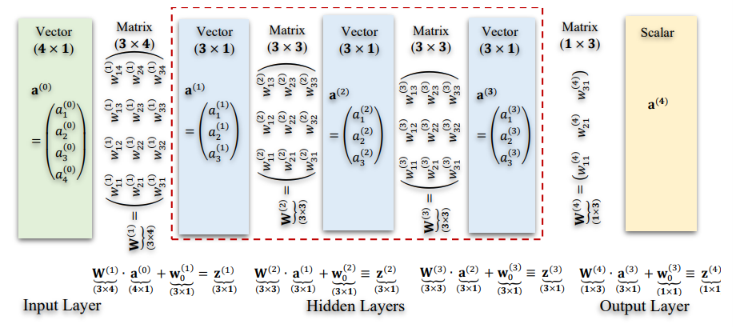
\includegraphics[width=\linewidth]{Images/04_Images/5.png}
    \caption{Kiến trúc cơ bản của một mạng nơ-ron truyền thẳng đa tầng}
    \label{4.5}
\end{figure}
Để minh họa quá trình lan truyền tiến một cách cụ thể, xét mạng nơ-ron truyền thẳng được trình bày trong Hình~\ref{4.5}, với cấu trúc $L = 4$ lớp, trong đó số lượng nơ-ron tại các lớp lần lượt là $n_0 = 4$, $n_1 = 3$, $n_2 = 3$, $n_3 = 3$ và $n_4 = 1$. Dựa trên cấu trúc này, quá trình lan truyền tiến qua từng lớp được biểu diễn như sau:
\paragraph{Lớp ẩn thứ nhất ($l = 1$)\\} 
\textbf{1. Tính véc-tơ tiền kích hoạt $\mathbf{z}^{[1]}$}
\begin{equation}
    \mathbf{z}^{[1]} = \mathbf{W}^{[1]} \mathbf{a}^{[0]} + \mathbf{w}_0^{[1]}
\end{equation}
Thay các ma trận trọng số và véc-tơ đầu vào, độ chệch cụ thể:
\begin{align}
    \begin{bmatrix} z_1^{[1]} \\ z_2^{[1]} \\ z_3^{[1]} \end{bmatrix} 
    &= \begin{bmatrix} 
        w_{11}^{[1]} & w_{12}^{[1]} & w_{13}^{[1]} & w_{14}^{[1]} \\ 
        w_{21}^{[1]} & w_{22}^{[1]} & w_{23}^{[1]} & w_{24}^{[1]} \\ 
        w_{31}^{[1]} & w_{32}^{[1]} & w_{33}^{[1]} & w_{34}^{[1]} 
    \end{bmatrix}
    \begin{bmatrix} a_1^{[0]} \\ a_2^{[0]} \\ a_3^{[0]} \\ a_4^{[0]} \end{bmatrix} 
    + \begin{bmatrix} w_{10}^{[1]} \\ w_{20}^{[1]} \\ w_{30}^{[1]} \end{bmatrix} \nonumber \\
    &= \begin{bmatrix}
        w_{11}^{[1]} a_1^{[0]} + w_{12}^{[1]} a_2^{[0]} + w_{13}^{[1]} a_3^{[0]} + w_{14}^{[1]} a_4^{[0]} \\
        w_{21}^{[1]} a_1^{[0]} + w_{22}^{[1]} a_2^{[0]} + w_{23}^{[1]} a_3^{[0]} + w_{24}^{[1]} a_4^{[0]} \\
        w_{31}^{[1]} a_1^{[0]} + w_{32}^{[1]} a_2^{[0]} + w_{33}^{[1]} a_3^{[0]} + w_{34}^{[1]} a_4^{[0]}
    \end{bmatrix}
    + \begin{bmatrix} w_{10}^{[1]} \\ w_{20}^{[1]} \\ w_{30}^{[1]} \end{bmatrix} \nonumber \\
    &= \begin{bmatrix} 
        w_{11}^{[1]} a_1^{[0]} + w_{12}^{[1]} a_2^{[0]} + w_{13}^{[1]} a_3^{[0]} + w_{14}^{[1]} a_4^{[0]} + w_{10}^{[1]} \\
        w_{21}^{[1]} a_1^{[0]} + w_{22}^{[1]} a_2^{[0]} + w_{23}^{[1]} a_3^{[0]} + w_{24}^{[1]} a_4^{[0]} + w_{20}^{[1]} \\
        w_{31}^{[1]} a_1^{[0]} + w_{32}^{[1]} a_2^{[0]} + w_{33}^{[1]} a_3^{[0]} + w_{34}^{[1]} a_4^{[0]} + w_{30}^{[1]} 
    \end{bmatrix}
\end{align}
\subparagraph{2. Tính véc-tơ kích hoạt đầu ra $\mathbf{a}^{[1]}$\\}
Áp dụng hàm kích hoạt phi tuyến $\sigma^{[1]}$ theo từng phần tử lên véc-tơ tiền kích hoạt:
\begin{equation}
    \mathbf{a}^{[1]} = \sigma^{[1]}\left(\mathbf{z}^{[1]}\right) 
    = \begin{bmatrix} a_1^{[1]} \\ a_2^{[1]} \\ a_3^{[1]} \end{bmatrix} 
    = \begin{bmatrix} 
        \sigma^{[1]}\left(z_1^{[1]}\right) \\ 
        \sigma^{[1]}\left(z_2^{[1]}\right) \\ 
        \sigma^{[1]}\left(z_3^{[1]}\right) 
    \end{bmatrix} \in \mathbb{R}^3
\end{equation}
Khai triển tường minh bằng cách thế trực tiếp các biểu thức $z_i^{[1]}$ vào hàm kích hoạt:
\begin{equation}
    \mathbf{a}^{[1]} = \begin{bmatrix} 
        \sigma^{[1]}\left( w_{11}^{[1]} a_1^{[0]} + w_{12}^{[1]} a_2^{[0]} + w_{13}^{[1]} a_3^{[0]} + w_{14}^{[1]} a_4^{[0]} + w_{10}^{[1]} \right) \\
        \sigma^{[1]}\left( w_{21}^{[1]} a_1^{[0]} + w_{22}^{[1]} a_2^{[0]} + w_{23}^{[1]} a_3^{[0]} + w_{24}^{[1]} a_4^{[0]} + w_{20}^{[1]} \right) \\
        \sigma^{[1]}\left( w_{31}^{[1]} a_1^{[0]} + w_{32}^{[1]} a_2^{[0]} + w_{33}^{[1]} a_3^{[0]} + w_{34}^{[1]} a_4^{[0]} + w_{30}^{[1]} \right)
    \end{bmatrix}
\end{equation}
Tương ứng với từng giá trị kích hoạt vô hướng:
\begin{equation}
    a_i^{[1]} = \sigma^{[1]}\left( \sum_{j=1}^{4} w_{ij}^{[1]} a_j^{[0]} + w_{i0}^{[1]} \right), \quad \forall i \in \{1, 2, 3\}.
\end{equation}

\paragraph{Lớp ẩn thứ hai ($l = 2$)\\} 
\textbf{1. Tính véc-tơ tiền kích hoạt $\mathbf{z}^{[2]}$}
\begin{equation}
    \mathbf{z}^{[2]} = \mathbf{W}^{[2]} \mathbf{a}^{[1]} + \mathbf{w}_0^{[2]}
\end{equation}
Thế các phần tử cụ thể của ma trận trọng số $\mathbf{W}^{[2]} \in \mathbb{R}^{3 \times 3}$, véc-tơ kích hoạt $\mathbf{a}^{[1]} \in \mathbb{R}^3$ từ lớp $l=1$, và véc-tơ độ chệch $\mathbf{w}_0^{[2]} \in \mathbb{R}^3$:
\begin{align}
    \begin{bmatrix} z_1^{[2]} \\ z_2^{[2]} \\ z_3^{[2]} \end{bmatrix} 
    &= \begin{bmatrix} 
        w_{11}^{[2]} & w_{12}^{[2]} & w_{13}^{[2]} \\ 
        w_{21}^{[2]} & w_{22}^{[2]} & w_{23}^{[2]} \\ 
        w_{31}^{[2]} & w_{32}^{[2]} & w_{33}^{[2]} 
    \end{bmatrix}
    \begin{bmatrix} a_1^{[1]} \\ a_2^{[1]} \\ a_3^{[1]} \end{bmatrix} 
    + \begin{bmatrix} w_{10}^{[2]} \\ w_{20}^{[2]} \\ w_{30}^{[2]} \end{bmatrix} \nonumber \\
    &= \begin{bmatrix}
        w_{11}^{[2]} a_1^{[1]} + w_{12}^{[2]} a_2^{[1]} + w_{13}^{[2]} a_3^{[1]} \\
        w_{21}^{[2]} a_1^{[1]} + w_{22}^{[2]} a_2^{[1]} + w_{23}^{[2]} a_3^{[1]} \\
        w_{31}^{[2]} a_1^{[1]} + w_{32}^{[2]} a_2^{[1]} + w_{33}^{[2]} a_3^{[1]}
    \end{bmatrix}
    + \begin{bmatrix} w_{10}^{[2]} \\ w_{20}^{[2]} \\ w_{30}^{[2]} \end{bmatrix} \nonumber \\
    &= \begin{bmatrix} 
        w_{11}^{[2]} a_1^{[1]} + w_{12}^{[2]} a_2^{[1]} + w_{13}^{[2]} a_3^{[1]} + w_{10}^{[2]} \\
        w_{21}^{[2]} a_1^{[1]} + w_{22}^{[2]} a_2^{[1]} + w_{23}^{[2]} a_3^{[1]} + w_{20}^{[2]} \\
        w_{31}^{[2]} a_1^{[1]} + w_{32}^{[2]} a_2^{[1]} + w_{33}^{[2]} a_3^{[1]} + w_{30}^{[2]} 
    \end{bmatrix}
\end{align}
\subparagraph{2. Tính véc-tơ kích hoạt đầu ra $\mathbf{a}^{[2]}$\\}
Áp dụng hàm kích hoạt phi tuyến $\sigma^{[2]}$ theo từng phần tử lên véc-tơ tiền kích hoạt $\mathbf{z}^{[2]}$:
\begin{equation}
    \mathbf{a}^{[2]} = \sigma^{[2]}\left(\mathbf{z}^{[2]}\right) 
    = \begin{bmatrix} a_1^{[2]} \\ a_2^{[2]} \\ a_3^{[2]} \end{bmatrix} 
    = \begin{bmatrix} 
        \sigma^{[2]}\left(z_1^{[2]}\right) \\ 
        \sigma^{[2]}\left(z_2^{[2]}\right) \\ 
        \sigma^{[2]}\left(z_3^{[2]}\right) 
    \end{bmatrix} \in \mathbb{R}^3
\end{equation}

Khai triển tường minh bằng cách thế trực tiếp các biểu thức $z_i^{[2]}$ vào hàm kích hoạt:
\begin{equation}
    \mathbf{a}^{[2]} = \begin{bmatrix} 
        \sigma^{[2]}\left( w_{11}^{[2]} a_1^{[1]} + w_{12}^{[2]} a_2^{[1]} + w_{13}^{[2]} a_3^{[1]} + w_{10}^{[2]} \right) \\
        \sigma^{[2]}\left( w_{21}^{[2]} a_1^{[1]} + w_{22}^{[2]} a_2^{[1]} + w_{23}^{[2]} a_3^{[1]} + w_{20}^{[2]} \right) \\
        \sigma^{[2]}\left( w_{31}^{[2]} a_1^{[1]} + w_{32}^{[2]} a_2^{[1]} + w_{33}^{[2]} a_3^{[1]} + w_{30}^{[2]} \right)
    \end{bmatrix}
\end{equation}

Dạng vô hướng cho từng nơ-ron:
\begin{equation}
    a_i^{[2]} = \sigma^{[2]}\left( \sum_{j=1}^{3} w_{ij}^{[2]} a_j^{[1]} + w_{i0}^{[2]} \right), \quad \forall i \in \{1, 2, 3\}.
\end{equation}
\paragraph{Lớp ẩn thứ ba ($l = 3$)\\} 
\textbf{1. Tính véc-tơ tiền kích hoạt $\mathbf{z}^{[3]}$}
\begin{equation}
    \mathbf{z}^{[3]} = \mathbf{W}^{[3]} \mathbf{a}^{[2]} + \mathbf{w}_0^{[3]}
\end{equation}
Thế các phần tử cụ thể của $\mathbf{W}^{[3]} \in \mathbb{R}^{3 \times 3}$, $\mathbf{a}^{[2]} \in \mathbb{R}^3$ và $\mathbf{w}_0^{[3]} \in \mathbb{R}^3$:
\begin{align}
    \begin{bmatrix} z_1^{[3]} \\ z_2^{[3]} \\ z_3^{[3]} \end{bmatrix} 
    &= \begin{bmatrix} 
        w_{11}^{[3]} & w_{12}^{[3]} & w_{13}^{[3]} \\ 
        w_{21}^{[3]} & w_{22}^{[3]} & w_{23}^{[3]} \\ 
        w_{31}^{[3]} & w_{32}^{[3]} & w_{33}^{[3]} 
    \end{bmatrix}
    \begin{bmatrix} a_1^{[2]} \\ a_2^{[2]} \\ a_3^{[2]} \end{bmatrix} 
    + \begin{bmatrix} w_{10}^{[3]} \\ w_{20}^{[3]} \\ w_{30}^{[3]} \end{bmatrix} \nonumber \\
    &= \begin{bmatrix}
        w_{11}^{[3]} a_1^{[2]} + w_{12}^{[3]} a_2^{[2]} + w_{13}^{[3]} a_3^{[2]} + w_{10}^{[3]} \\
        w_{21}^{[3]} a_1^{[2]} + w_{22}^{[3]} a_2^{[2]} + w_{23}^{[3]} a_3^{[2]} + w_{20}^{[3]} \\
        w_{31}^{[3]} a_1^{[2]} + w_{32}^{[3]} a_2^{[2]} + w_{33}^{[3]} a_3^{[2]} + w_{30}^{[3]} 
    \end{bmatrix}
\end{align}
\subparagraph{2. Tính véc-tơ kích hoạt đầu ra $\mathbf{a}^{[3]}$\\}
Áp dụng hàm kích hoạt $\sigma^{[3]}$ theo từng phần tử:
\begin{equation}
    \mathbf{a}^{[3]} = \sigma^{[3]}\left(\mathbf{z}^{[3]}\right) 
    = \begin{bmatrix} 
        \sigma^{[3]}\left(z_1^{[3]}\right) \\ 
        \sigma^{[3]}\left(z_2^{[3]}\right) \\ 
        \sigma^{[3]}\left(z_3^{[3]}\right) 
    \end{bmatrix} 
    = \begin{bmatrix} 
        \sigma^{[3]}\left( \sum_{j=1}^{3} w_{1j}^{[3]} a_j^{[2]} + w_{10}^{[3]} \right) \\
        \sigma^{[3]}\left( \sum_{j=1}^{3} w_{2j}^{[3]} a_j^{[2]} + w_{20}^{[3]} \right) \\
        \sigma^{[3]}\left( \sum_{j=1}^{3} w_{3j}^{[3]} a_j^{[2]} + w_{30}^{[3]} \right)
    \end{bmatrix} \in \mathbb{R}^3
\end{equation}
\paragraph{Lớp đầu ra ($l = 4$)\\} 
\textbf{1. Tính giá trị tiền kích hoạt $z^{[4]}$}
\begin{equation}
    z^{[4]} = \mathbf{W}^{[4]} \mathbf{a}^{[3]} + \mathbf{w}_0^{[4]}
\end{equation}
Với ma trận trọng số $\mathbf{W}^{[4]} \in \mathbb{R}^{1 \times 3}$ và độ chệch $\mathbf{w}_0^{[4]} \in \mathbb{R}^1$:
\begin{align}
    \left[ z_1^{[4]} \right] 
    &= \begin{bmatrix} w_{11}^{[4]} & w_{12}^{[4]} & w_{13}^{[4]} \end{bmatrix}
    \begin{bmatrix} a_1^{[3]} \\ a_2^{[3]} \\ a_3^{[3]} \end{bmatrix} 
    + \left[ w_{10}^{[4]} \right] \nonumber \\
    &= \left[ w_{11}^{[4]} a_1^{[3]} + w_{12}^{[4]} a_2^{[3]} + w_{13}^{[4]} a_3^{[3]} + w_{10}^{[4]} \right] \nonumber \\
    &= \left[ \sum_{j=1}^{3} w_{1j}^{[4]} a_j^{[3]} + w_{10}^{[4]} \right]
\end{align}
\subparagraph{2. Tính giá trị dự đoán $a^{[4]}$\\}
\begin{equation}
    a^{[4]} = \sigma^{[4]}\left(z^{[4]}\right) 
    = \left[ \sigma^{[4]}\left( \sum_{j=1}^{3} w_{1j}^{[4]} a_j^{[3]} + w_{10}^{[4]} \right) \right] \in \mathbb{R}^1
\end{equation}
Dưới góc nhìn hình học vi phân và đại số tuyến tính, mỗi lớp của mạng nơ-ron thực chất là một phép biến đổi tuyến tính cùng một phép biến đổi phi tuyến theo từng tọa độ. Do đó, toàn bộ mạng nơ-ron sâu $L$ lớp có thể được trừu tượng hóa thành một hàm hợp $\mathcal{N}$ ánh xạ giữa hai không gian Euclid:
\begin{equation}
    \mathcal{N}: \mathbb{R}^{n_0} \to \mathbb{R}^{n_L}
\end{equation}

Hàm $\mathcal{N}$ được biểu diễn tường minh dưới dạng chuỗi các hàm hợp lồng nhau:
\begin{equation}
    \mathcal{N}(\mathbf{a}^{[0]}) = (\mathbf{f}^{[L]} \circ \mathbf{f}^{[L-1]} \circ \dots \circ \mathbf{f}^{[1]})(\mathbf{a}^{[0]})
\end{equation}
trong đó mỗi phép biến đổi lớp $\mathbf{f}^{[l]}: \mathbb{R}^{n_{l-1}} \to \mathbb{R}^{n_l}$ được xác định bởi:
\begin{equation}
    \mathbf{f}^{[l]}(\mathbf{a}^{[l-1]}) = \sigma^{[l]}\left(\mathbf{W}^{[l]} \mathbf{a}^{[l-1]} + \mathbf{w}_0^{[l]}\right), \quad \forall l \in \{1, 2, \dots, L\}
\end{equation}

Đối với kiến trúc mạng $4$ lớp cụ thể đang xét, ánh xạ thu về trường hợp $\mathcal{N}: \mathbb{R}^4 \to \mathbb{R}^1$. Phương trình hàm hợp được biểu diễn như sau:
\begin{equation}
\resizebox{0.96\linewidth}{!}{$
    \mathcal{N}\left(\mathbf{a}^{[0]}\right) = \sigma^{[4]} \left( \mathbf{W}^{[4]} \sigma^{[3]} \left( \mathbf{W}^{[3]} \sigma^{[2]} \left( \mathbf{W}^{[2]} \sigma^{[1]} \left( \mathbf{W}^{[1]} \mathbf{a}^{[0]} + \mathbf{w}_0^{[1]} \right) + \mathbf{w}_0^{[2]} \right) + \mathbf{w}_0^{[3]} \right) + \mathbf{w}_0^{[4]} \right) = \mathbf{a}^{[4]}
$}
\end{equation}
trong đó các biến trạng thái trung gian và số chiều không gian tương ứng tại mỗi lớp được xác định bởi các hệ thức sau:
\begin{align}
    \mathbf{z}^{[1]} &= \underbrace{\mathbf{W}^{[1]}}_{3 \times 4} \underbrace{\mathbf{a}^{[0]}}_{4 \times 1} + \underbrace{\mathbf{w}_0^{[1]}}_{3 \times 1} \in \mathbb{R}^3, \quad 
    &&\mathbf{a}^{[1]} = \sigma^{[1]}\left(\mathbf{z}^{[1]}\right) \in \mathbb{R}^3, \\
    \mathbf{z}^{[2]} &= \underbrace{\mathbf{W}^{[2]}}_{3 \times 3} \underbrace{\mathbf{a}^{[1]}}_{3 \times 1} + \underbrace{\mathbf{w}_0^{[2]}}_{3 \times 1} \in \mathbb{R}^3, \quad 
    &&\mathbf{a}^{[2]} = \sigma^{[2]}\left(\mathbf{z}^{[2]}\right) \in \mathbb{R}^3, \\
    \mathbf{z}^{[3]} &= \underbrace{\mathbf{W}^{[3]}}_{3 \times 3} \underbrace{\mathbf{a}^{[2]}}_{3 \times 1} + \underbrace{\mathbf{w}_0^{[3]}}_{3 \times 1} \in \mathbb{R}^3, \quad 
    &&\mathbf{a}^{[3]} = \sigma^{[3]}\left(\mathbf{z}^{[3]}\right) \in \mathbb{R}^3, \\
    \mathbf{z}^{[4]} &= \underbrace{\mathbf{W}^{[4]}}_{1 \times 3} \underbrace{\mathbf{a}^{[3]}}_{3 \times 1} + \underbrace{\mathbf{w}_0^{[4]}}_{1 \times 1} \in \mathbb{R}^1, \quad 
    &&\mathbf{a}^{[4]} = \sigma^{[4]}\left(\mathbf{z}^{[4]}\right) \in \mathbb{R}^1.
\end{align}

\begin{remark}
Mạng nơ-ron sâu có thể được xem như một toán tử tham số hóa, được xây dựng thông qua phép hợp của một chuỗi các ánh xạ liên tiếp. Toán tử này được xác định bởi tập tham số:
\[\boldsymbol{\theta} 
= \left\{\mathbf{W}^{[l]},
\mathbf{b}^{[l]} \right\}_{l=1}^{L}.\]
Khả năng biểu diễn các ánh xạ phức tạp của mạng phụ thuộc đồng thời vào cấu trúc kiến trúc và giá trị của tập tham số $\boldsymbol{\theta}$.
\end{remark}
    % \item Đối với một số mô hình thống kê tuyến tính cổ điển, chẳng hạn mô hình hồi quy theo phương pháp bình phương tối thiểu, nghiệm tối ưu của tham số có thể được xác định thông qua công thức giải tích dạng đóng:
    % \[
    %     \mathbf{w}^{*}
    %     =
    %     \left(\mathbf{X}^{\top}\mathbf{X}\right)^{-1}
    %     \mathbf{X}^{\top}\mathbf{y},
    %     \qquad
    %     \text{khi }
    %     \mathbf{X}^{\top}\mathbf{X}
    %     \text{ khả nghịch}.
    % \]
    % Ngược lại, đối với mạng nơ-ron nhiều lớp, hàm mất mát nói chung là một hàm phi tuyến và không lồi theo tập tham số. Vì vậy, nghiệm tối ưu thường không thể biểu diễn dưới dạng công thức giải tích dạng đóng. Việc xác định các tham số phù hợp do đó thường được thực hiện bằng các phương pháp tối ưu hóa số lặp, chẳng hạn phương pháp hạ dốc theo hướng giảm của hàm mất mát và các biến thể của phương pháp này.

\paragraph{Ví dụ tính toán lan truyền tiến cho một mẫu dữ liệu.}
Xét mạng nơ-ron truyền thẳng 4 lớp với kiến trúc:
\begin{itemize}
    \item \textbf{Lớp đầu vào ($l=0$):} $n_0 = 3$ đặc trưng.
    \item \textbf{Lớp ẩn 1 ($l=1$):} $n_1 = 3$ nơ-ron, hàm kích hoạt ReLU.
    \item \textbf{Lớp ẩn 2 ($l=2$):} $n_2 = 3$ nơ-ron, hàm kích hoạt ReLU.
    \item \textbf{Lớp ẩn 3 ($l=3$):} $n_3 = 3$ nơ-ron, hàm kích hoạt ReLU.
    \item \textbf{Lớp đầu ra ($l=4$):} $n_4 = 1$ nơ-ron, hàm kích hoạt ReLU.
\end{itemize}
\paragraph{Khởi tạo Dữ liệu và Tham số:}
Véc-tơ đầu vào $\mathbf{x} = \mathbf{a}^{[0]} \in \mathbb{R}^{3 \times 1}$:
\begin{equation}
\mathbf{a}^{[0]} = 
\begin{bmatrix}
    1 \\ 0 \\ -1
\end{bmatrix}
\end{equation}

Trọng số và độ chệch tại \textbf{Lớp 1}:
\begin{equation}
\mathbf{W}^{[1]} = 
\begin{bmatrix}
    1 & 0 & -1 \\
    0 & 1 & 1 \\
    -1 & -1 & 0
\end{bmatrix}, 
\quad
\mathbf{b}^{[1]} = 
\begin{bmatrix}
    0 \\ -1 \\ 1
\end{bmatrix}
\end{equation}

Trọng số và độ chệch tại \textbf{Lớp 2}:
\begin{equation}
\mathbf{W}^{[2]} = 
\begin{bmatrix}
    1 & -1 & 0 \\
    0 & 1 & 2 \\
    -1 & 0 & 1
\end{bmatrix}, 
\quad
\mathbf{b}^{[2]} = 
\begin{bmatrix}
    1 \\ -2 \\ 0
\end{bmatrix}
\end{equation}

Trọng số và độ chệch tại \textbf{Lớp 3}:
\begin{equation}
\mathbf{W}^{[3]} = 
\begin{bmatrix}
    -1 & 1 & 0 \\
    1 & 0 & -1 \\
    0 & 2 & 1
\end{bmatrix}, 
\quad
\mathbf{b}^{[3]} = 
\begin{bmatrix}
    2 \\ -1 \\ 1
\end{bmatrix}
\end{equation}

Trọng số và độ chệch tại \textbf{Lớp Đầu ra (Lớp 4)}:
\begin{equation}
\mathbf{W}^{[4]} = 
\begin{bmatrix}
    1 & 2 & -1
\end{bmatrix},
\quad
\mathbf{b}^{[4]} = 
\begin{bmatrix}
    -1
\end{bmatrix}
\end{equation}

\paragraph{Tại lớp ẩn 1 ($l=1$):\\}
Tính $\mathbf{z}^{[1]} = \mathbf{W}^{[1]}\mathbf{a}^{[0]} + \mathbf{b}^{[1]}$
\begin{align*}
\mathbf{W}^{[1]}\mathbf{a}^{[0]} 
&= 
\begin{bmatrix}
    1 & 0 & -1 \\
    0 & 1 & 1 \\
    -1 & -1 & 0
\end{bmatrix}
\begin{bmatrix}
    1 \\ 0 \\ -1
\end{bmatrix}
=
\begin{bmatrix}
    (1\cdot 1 + 0\cdot 0 - 1\cdot -1) \\
    (0\cdot 1 + 1\cdot 0 + 1\cdot -1) \\
    (-1\cdot 1 - 1\cdot 0 + 0\cdot -1)
\end{bmatrix}
=
\begin{bmatrix}
    2 \\ -1 \\ -1
\end{bmatrix}
\end{align*}
\begin{equation}
\mathbf{z}^{[1]} = 
\begin{bmatrix}
    2 \\ -1 \\ -1
\end{bmatrix}
+
\begin{bmatrix}
    0 \\ -1 \\ 1
\end{bmatrix}
=
\begin{bmatrix}
    2 \\ -2 \\ 0
\end{bmatrix}
\end{equation}
\begin{equation}
\mathbf{a}^{[1]} = 
\begin{bmatrix}
    \max(0, 2) \\
    \max(0, -2) \\
    \max(0, 0)
\end{bmatrix}
=
\begin{bmatrix}
    2 \\ 0 \\ 0
\end{bmatrix}
\end{equation}

\paragraph{Tại lớp ẩn 2 ($l=2$):\\}
\textbf{Tính $\mathbf{z}^{[2]} = \mathbf{W}^{[2]}\mathbf{a}^{[1]} + \mathbf{b}^{[2]}$}
\begin{align*}
\mathbf{W}^{[2]}\mathbf{a}^{[1]} 
&= 
\begin{bmatrix}
    1 & -1 & 0 \\
    0 & 1 & 2 \\
    -1 & 0 & 1
\end{bmatrix}
\begin{bmatrix}
    2 \\ 0 \\ 0
\end{bmatrix}
=
\begin{bmatrix}
    (1\cdot 2 - 1\cdot 0 + 0\cdot 0) \\
    (0\cdot 2 + 1\cdot 0 + 2\cdot 0) \\
    (-1\cdot 2 + 0\cdot 0 + 1\cdot 0)
\end{bmatrix}
=
\begin{bmatrix}
    2 \\ 0 \\ -2
\end{bmatrix}
\end{align*}
\begin{equation}
\mathbf{z}^{[2]} = 
\begin{bmatrix}
    2 \\ 0 \\ -2
\end{bmatrix}
+
\begin{bmatrix}
    1 \\ -2 \\ 0
\end{bmatrix}
=
\begin{bmatrix}
    3 \\ -2 \\ -2
\end{bmatrix}
\end{equation}

\begin{equation}
\mathbf{a}^{[2]} = 
\begin{bmatrix}
    \max(0, 3) \\
    \max(0, -2) \\
    \max(0, -2)
\end{bmatrix}
=
\begin{bmatrix}
    3 \\ 0 \\ 0
\end{bmatrix}
\end{equation}

\paragraph{Tại lớp ẩn 3 ($l=3$):\\}
\textbf{Tính $\mathbf{z}^{[3]} = \mathbf{W}^{[3]}\mathbf{a}^{[2]} + \mathbf{b}^{[3]}$}
\begin{align*}
\mathbf{W}^{[3]}\mathbf{a}^{[2]} 
&= 
\begin{bmatrix}
    -1 & 1 & 0 \\
    1 & 0 & -1 \\
    0 & 2 & 1
\end{bmatrix}
\begin{bmatrix}
    3 \\ 0 \\ 0
\end{bmatrix}
=
\begin{bmatrix}
    (-1\cdot 3 + 1\cdot 0 + 0\cdot 0) \\
    (1\cdot 3 + 0\cdot 0 - 1\cdot 0) \\
    (0\cdot 3 + 2\cdot 0 + 1\cdot 0)
\end{bmatrix}
=
\begin{bmatrix}
    -3 \\ 3 \\ 0
\end{bmatrix}
\end{align*}
\begin{equation}
\mathbf{z}^{[3]} = 
\begin{bmatrix}
    -3 \\ 3 \\ 0
\end{bmatrix}
+
\begin{bmatrix}
    2 \\ -1 \\ 1
\end{bmatrix}
=
\begin{bmatrix}
    -1 \\ 2 \\ 1
\end{bmatrix}
\end{equation}

\begin{equation}
\mathbf{a}^{[3]} = 
\begin{bmatrix}
    \max(0, -1) \\
    \max(0, 2) \\
    \max(0, 1)
\end{bmatrix}
=
\begin{bmatrix}
    0 \\ 2 \\ 1
\end{bmatrix}
\end{equation}

\paragraph{Tại lớp đầu ra ($l=4$):\\}
\textbf{Tính $z^{[4]} = \mathbf{W}^{[4]}\mathbf{a}^{[3]} + b^{[4]}$}
\begin{align*}
\mathbf{W}^{[4]}\mathbf{a}^{[3]} 
&= 
\begin{bmatrix}
    1 & 2 & -1
\end{bmatrix}
\begin{bmatrix}
    0 \\ 2 \\ 1
\end{bmatrix}
=
1\cdot 0 + 2\cdot 2 - 1\cdot 1 = 3
\end{align*}
\begin{equation}
z^{[4]} = 3 + (-1) = 2
\end{equation}
\begin{equation}
\hat{y} = a^{[4]} = \max(0, 2) = 2
\end{equation}

\paragraph{Kết luận:} 
Với mẫu dữ liệu đầu vào $\mathbf{x} = [1, 0, -1]^\top$, mạng nơ-ron đã đưa ra giá trị dự đoán cuối cùng là $\hat{y} = 2$. 

\begin{lstlisting}[caption={Mã Python cho lan truyền tiến của một mẫu dữ liệu.}, language=Python]
import numpy as np

# --- ReLU ---
def relu(z: np.ndarray) -> np.ndarray:
    return np.maximum(0, z)

# --- Khoi tao du lieu ---
a0 = np.array([[1], [0], [-1]])

# Tham so Lop 1
W1 = np.array([[1, 0, -1], [0, 1, 1], [-1, -1, 0]])
b1 = np.array([[0], [-1], [1]])

# Tham so Lop 2
W2 = np.array([[1, -1, 0], [0, 1, 2], [-1, 0, 1]])
b2 = np.array([[1], [-2], [0]])

# Tham so Lop 3
W3 = np.array([[-1, 1, 0], [1, 0, -1], [0, 2, 1]])
b3 = np.array([[2], [-1], [1]])

# Tham so Lop 4 (Dau ra)
W4 = np.array([[1, 2, -1]])
b4 = np.array([[-1]])

# --- Lan truyen tien ---
def forward() -> None:
    # Lop 1
    z1 = W1 @ a0 + b1
    a1 = relu(z1)

    # Lop 2
    z2 = W2 @ a1 + b2
    a2 = relu(z2)

    # Lop 3
    z3 = W3 @ a2 + b3
    a3 = relu(z3)

    # Lop 4
    z4 = W4 @ a3 + b4
    y_hat = relu(z4)

    # In ket qua
    print("a_1:\n", a1)
    print("a_2:\n", a2)
    print("a_3:\n", a3)
    print("y_hat:\n", y_hat)

if __name__ == "__main__":
    forward()


\end{lstlisting}